\begin{FPfigure}

\begin{center}
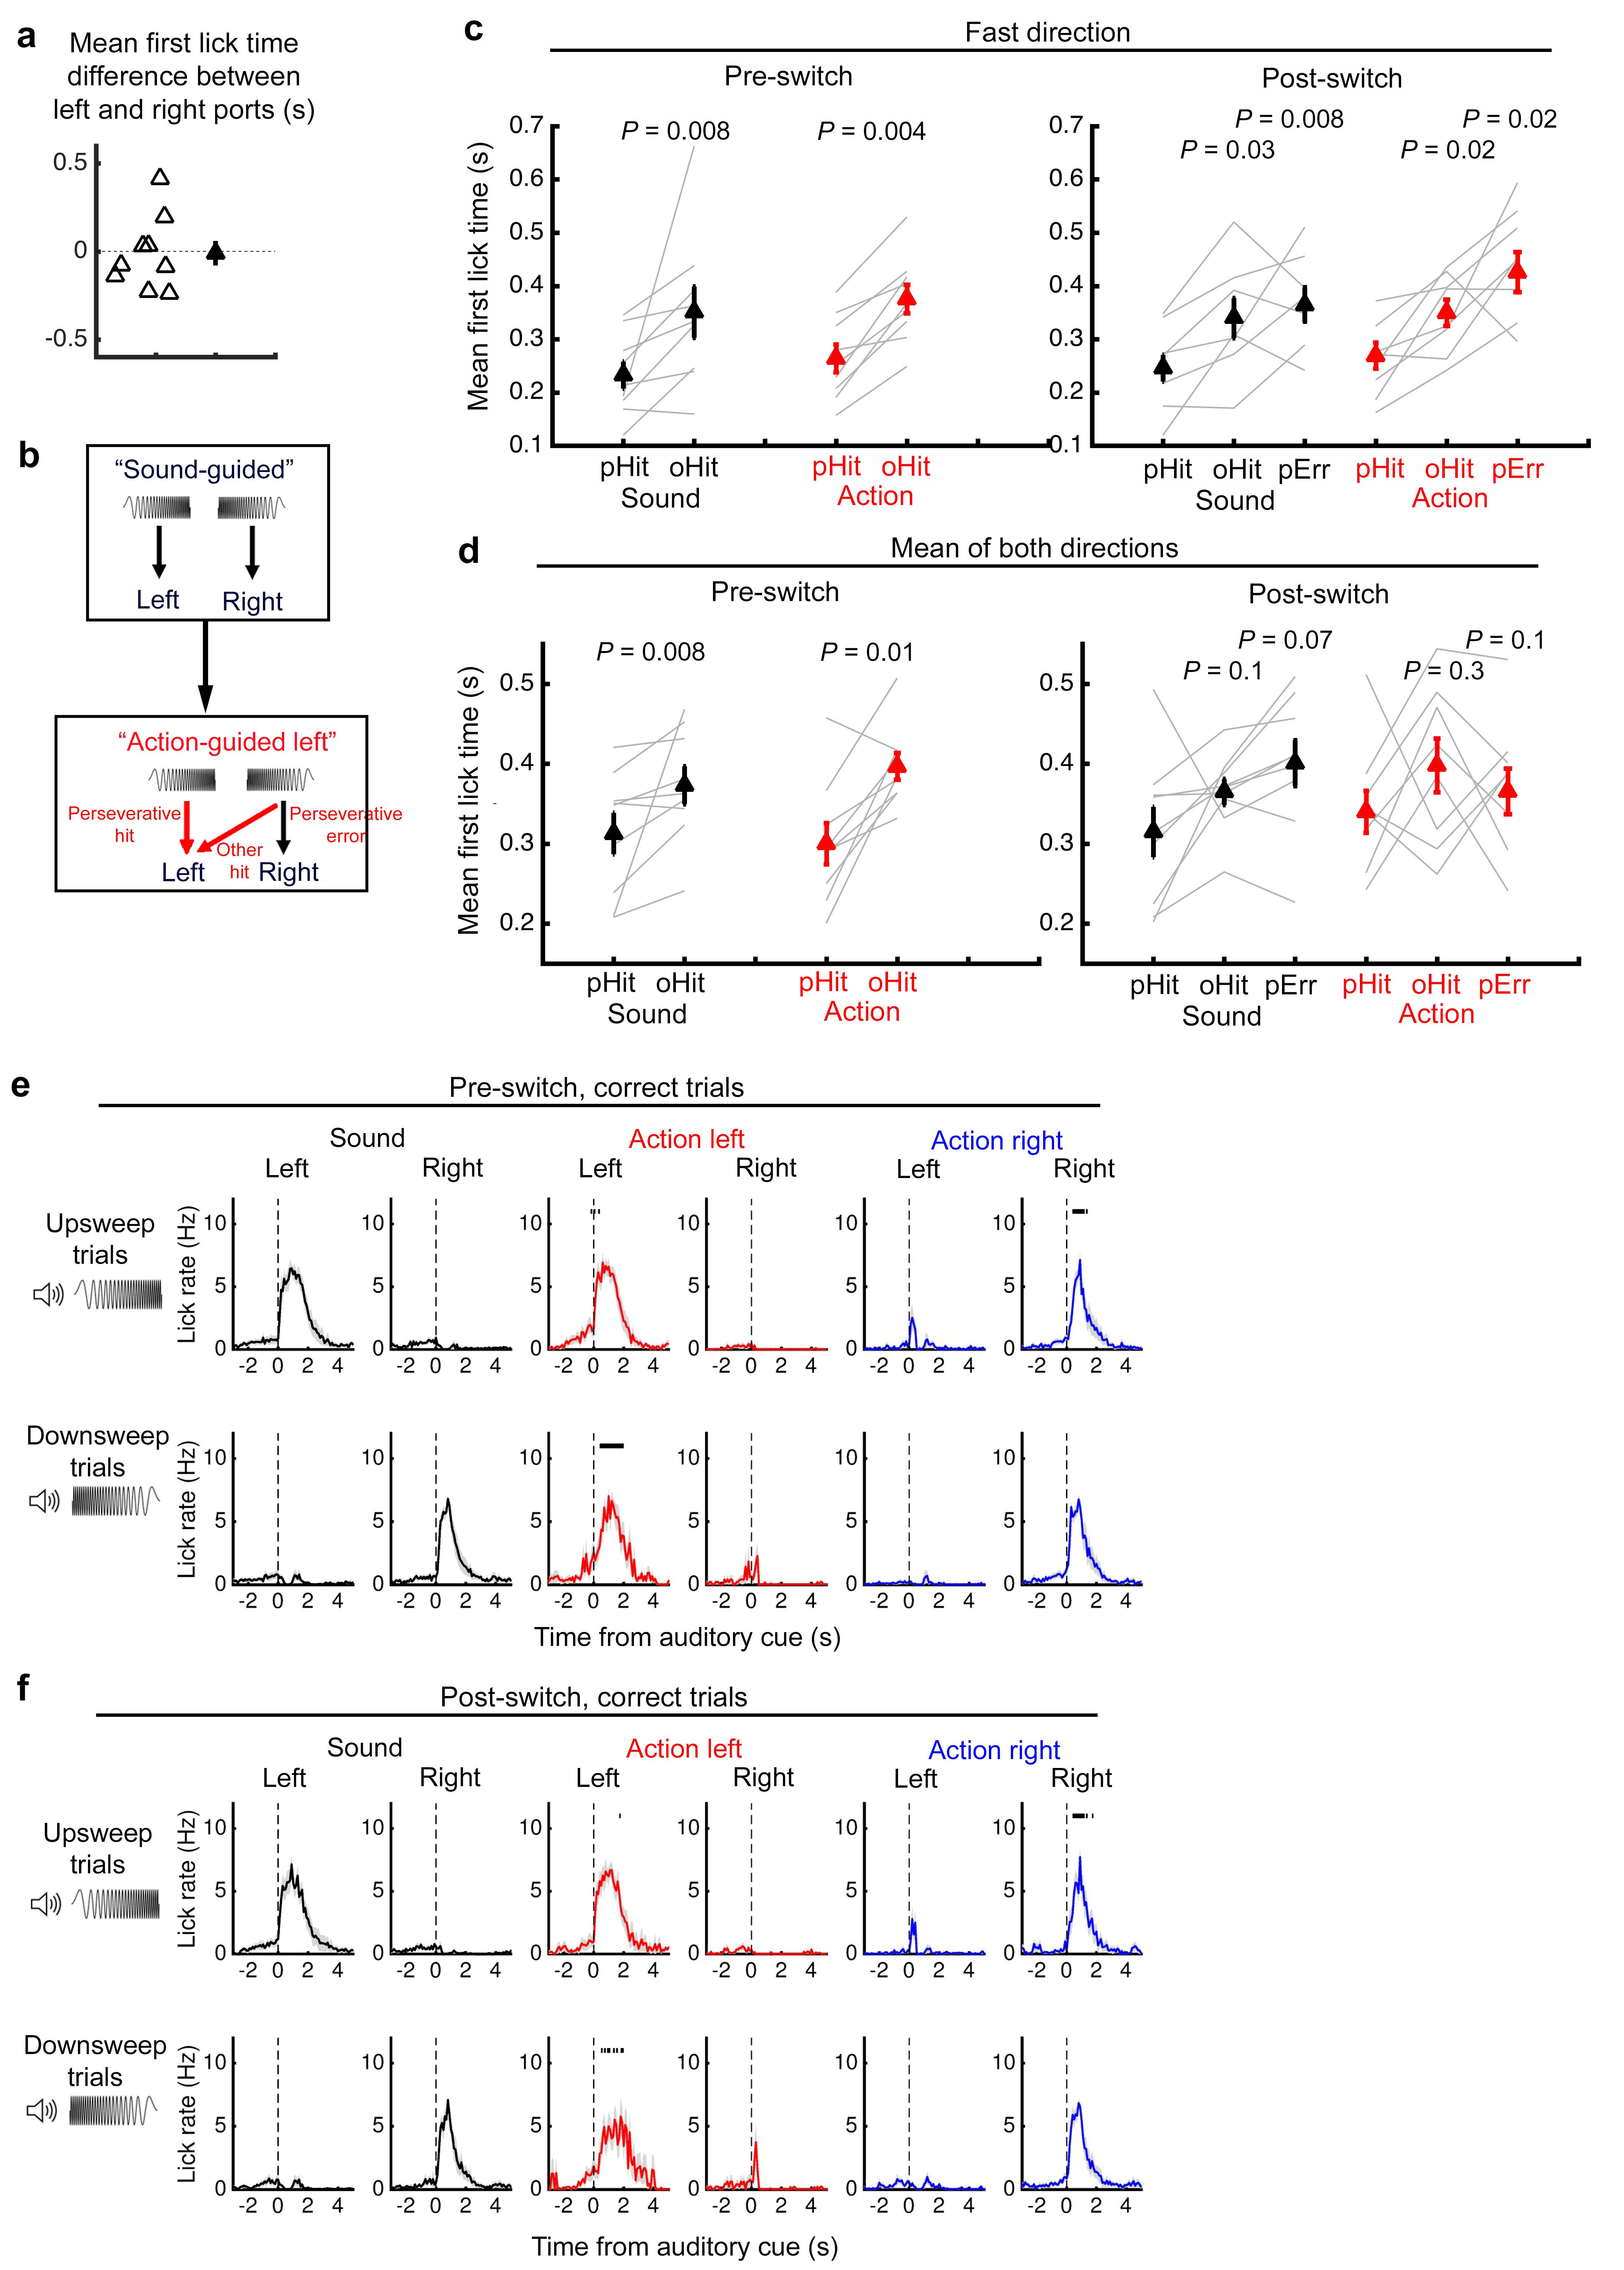
\includegraphics[width=\textwidth]{Figures/Chapter3/NN_figS2} \end{center}

\footnotesize{Figure \ref{fig:NN_figS2}: Slower response times in trials incongruent with the stimulus–-response contingencies of the prior block.}

\caption[Slower response times in trials incongruent with the stimulus–-response contingencies of the prior block]
{Slower first lick times in trials that were incongruent with the stimulus-–response contingencies of the prior block.
(a) The difference in mean response times (see Methods for definition) between left and right choices for perseverative hit trials during sound blocks. Open triangle, individual experiment. Filled triangle, $\mathit{mean}\pm\mathit{SEM}$. This plot shows that a mouse could respond faster to at either the left or right lick port. The differences could be due to a combination of factors including placement of the lick ports and the internal bias of the animal. (b) Schematic illustrating perseverative hit, other hit, and perseverative error trials. (c) Based on the analysis in \emph{a}, either left or right is denoted as the fast direction. The mean response times for the fast direction are plotted for perseverative hit (pHit), other hit (oHit), and perseverative error (pErr) trials occurring during pre-switch (20 trials before block switch) or post-switch (20 trials after block switch) condition. The Wilcoxon signed-rank test was used to assess differences between pHit trials and oHit or pErr trials in the same block type. We also tested sound versus action blocks, and found no significant differences for any comparisons of the same trial types ($p>0.05$, Wilcoxon signed-rank test). Line, individual experiments. Filled triangles, $\mathit{mean}\pm\mathit{SEM}$ (d) Same as \emph{c} presenting the grand mean response time for the fast and slow directions for each experiment. There were no significant differences for any comparisons of the same trial types between sound and action blocks ($p>0.05$, Wilcoxon signed-rank test). (e) Same as Fig. \ref{fig:NN_fig1}e, limited to the 20 trials pre-switch. (f) Same as Fig. \ref{fig:NN_fig1}e, limited to the 20 trials post-switch. $N = 9$ sessions from 5 mice.}

\label{fig:NN_figS2}
\end{FPfigure}
